\documentclass[11pt]{article}
\input{glyphtounicode}
\input{glyphtounicode-cmex}
\pdfgentounicode=1
\usepackage[T1]{fontenc}
\usepackage[utf8]{inputenc}
\usepackage{lmodern,amsmath,amssymb,amsthm,mathtools}
\usepackage[margin=1in]{geometry}
\usepackage{microtype,tikz,needspace}
\usetikzlibrary{arrows.meta,calc}
\usepackage[hidelinks]{hyperref}
\hypersetup{pdftitle={The Kervaire theorem for groups},pdfauthor={OpenAI}}
\usepackage[nameinlink,capitalise,noabbrev]{cleveref}
\newtheorem{theorem}{Theorem}[section]
\newtheorem{lemma}[theorem]{Lemma}
\newtheorem{proposition}[theorem]{Proposition}
\newtheorem{corollary}[theorem]{Corollary}
\theoremstyle{definition}
\newtheorem{remark}[theorem]{Remark}
\newcommand{\C}{\mathbb C}
\newcommand{\Z}{\mathbb Z}
\newcommand{\R}{\mathbb R}
\newcommand{\T}{\mathbb T}
\DeclareMathOperator{\U}{U}
\DeclareMathOperator{\Gr}{Gr}
\DeclareMathOperator{\diag}{diag}
\DeclareMathOperator{\Tr}{Tr}
\DeclareMathOperator{\Ad}{Ad}
\title{The Kervaire theorem for groups}
\author{OpenAI}
\date{September 24, 2026}
\begin{document}
\maketitle
\begin{abstract}
We prove that no free product of a nontrivial group with an infinite cyclic
group is normally generated by one element. This resolves the Kervaire
conjecture positively.
\end{abstract}
\tableofcontents
\section{Introduction}

Adding one generator and one relation to a nontrivial group should leave
a nontrivial group. This is the Kervaire conjecture. We prove it by
establishing coefficient injectivity in the case where the new generator
has exponent sum $\pm1$.

Let $A$ be a group, let $\langle t\rangle\cong\Z$, and set
$H=A*\langle t\rangle$. Write $p:H\to\Z$ for the homomorphism that kills
$A$ and sends $t$ to $1$. A word $w\in H$ is \emph{unimodular} if
$p(w)=\pm1$. Denote its normal closure in $H$ by
$\langle\!\langle w\rangle\!\rangle_H$.

The equation $w(t)=1$ is \emph{solvable over $A$} if there are an
embedding $A\to B$ and an element $b\in B$ such that evaluating $t$ at
$b$ gives $w(b)=1$. This is equivalent to injectivity of the coefficient
map $A\to H/\langle\!\langle w\rangle\!\rangle_H$: every solution
factors through this quotient, while an injective coefficient map lets
the quotient itself supply a solution.

\Needspace{7\baselineskip}
\begin{samepage}
\begin{theorem}\label{thm:main}
For every group $A$ and every unimodular word $w\in A*\langle t\rangle$,
the canonical homomorphism
\[
 A\longrightarrow (A*\langle t\rangle)/\langle\!\langle w\rangle\!\rangle_H
\]
is injective.
\end{theorem}
\end{samepage}

No restriction on torsion, cardinality, or presentation of $A$ is imposed.
The nontriviality assertion for all exponent sums follows at once.

\begin{corollary}[The Kervaire conjecture]\label{cor:kervaire}
If $A\ne1$, then
$(A*\langle t\rangle)/\langle\!\langle w\rangle\!\rangle_H\ne1$
for every $w\in A*\langle t\rangle$.
\end{corollary}
\begin{proof}
For $p(w)=\pm1$, apply Theorem~\ref{thm:main}.
For every other integer $d=p(w)$, the map $p$ induces a surjection from
the quotient onto the nontrivial group $\Z/d\Z$, where $\Z/0\Z=\Z$.
\end{proof}

\subsection{Context and methods}

Kervaire's characterization of high-dimensional knot groups includes
normal generation by a single element \cite[Theorem 1.1]{Kervaire1965}.
Chen \cite[preprint Section 1]{Chen2026} traces the group-theoretic
Kervaire problem to this setting. Its stronger Kervaire--Laudenbach form
asks for coefficient injectivity whenever $p(w)\ne0$; such one-variable
equations are called \emph{nonsingular}. Theorem~\ref{thm:main} proves its
unimodular case, while Corollary~\ref{cor:kervaire} resolves the full
nontriviality conjecture.
At the level of assertions for all groups, this nontriviality statement
is equivalent to unimodular coefficient injectivity: Klyachko records the
standard reduction through an embedding into a simple group
\cite[preprint Section 3, Proposition 2]{Klyachko2004}.
We prove injectivity directly.

Gerstenhaber and Rothaus proved solvability of nonsingular systems of
equations over finite groups in finite overgroups
\cite[Theorem 2]{GerstenhaberRothaus1962}.
In particular their theorem gives the required injectivity for finite
coefficient groups, and hence for residually finite groups by separating
each nonidentity coefficient in a finite quotient.
Pestov records the resulting ultraproduct extension: nonsingular
equations over hyperlinear groups have solutions in hyperlinear
overgroups \cite[preprint Corollary 10.4]{Pestov2008}.
Hyperlinear groups admit embeddings into metric ultraproducts of unitary
groups with normalized Hilbert--Schmidt metrics.
Klyachko proved unimodular injectivity for torsion-free groups
\cite[Theorem 4, exponent-one case]{Klyachko1993}. Chen gave a new proof
through estimates for the complexity of surfaces
\cite[preprint Theorem 6.9]{Chen2026}. For arbitrary coefficient groups,
Klyachko and Lurye proved injectivity after imposing $w^m=1$ when $w$ is
unimodular and $m\geq2$
\cite[preprint Section 1, Theorem; Section 5]{KlyachkoLurye2012}; this does not impose
$w=1$.

Kawauchi has published a proposed resolution of the universal
nontriviality assertion through knot exteriors, relative collapses, and
ribbon sphere-link groups \cite[Theorem 1 and Corollary 2]{Kawauchi2024}.
By the equivalence just recalled, its endpoint includes unimodular
injectivity. The argument below takes a different route through spectral
phase and a finite-dimensional fixed-space theorem; neither the collapse
construction nor the ribbon-asphericity assertions enter its proof.
Recent work of Klyachko, Mikheenko, and Olshanskii also distinguishes
solvability inside a coefficient group from solvability in an overgroup
\cite[Sections 1 and 3]{KlyachkoMikheenkoOlshanskii2026}.
Our conclusion concerns the latter and does not assert that a solution
already lies in $A$.

Unitary groups and degree theory already play a central role in the
Gerstenhaber--Rothaus method \cite[Theorem 1]{GerstenhaberRothaus1962}; see also
\cite[Section 1.1]{KlyachkoThom2017}.
Corner-labelled diagrams and Euler-characteristic estimates likewise
have a substantial history in equations over groups
\cite[preprint Sections 3--4]{KlyachkoLurye2012}
and \cite[preprint Sections 2--4]{Chen2026}.
Here these methods meet through a trace comparison for permutations
weighted by the left regular representation of $A$. The regular
representation is available for every group and supplies a faithful
finite trace without an approximation hypothesis on $A$.
For the spectral ingredient, Thompson's matrix exponential formula and
its extensions provide a related precedent
\cite[Section 2 and Theorem 4.4]{AntezanaLarotondaVarela2012};
Section~\ref{sec:phase} distinguishes those formulas from the unrestricted
phase inequality proved here.

Two ingredients are useful independently of the diagram argument.
The first is subadditivity of the trace of the fractional spectral phase
of a unitary. The second is a fixed-space lemma: given $k\geq1$, signs
$s_1,\ldots,s_n\in\{1,-1\}$ with $\sum_i s_i=\pm1$, and $P\in\U(nk)$,
some $X\in\U(k)$ makes $\diag(X^{s_1},\ldots,X^{s_n})P$
have at least $k$ fixed directions. We prove the latter by a degree
calculation on a compact manifold that records a unitary together with
a fixed $k$-plane. Their combination gives the planar obstruction below.

\subsection{Proof overview}

Suppose a coefficient $g\in A$ becomes trivial after imposing $w=1$.
A finite expression for $g$ as a product of conjugates of $w$ and $w^{-1}$
can be drawn on a punctured disk. Pairing the occurrences of $t$ produces
disjoint bands between word disks. The complementary boundary curves
read words in $A$.

The central assertion is Theorem~\ref{thm:planar}: in a connected planar
surface made from these disks and bands, one boundary word cannot be the
only nontrivial one. To prove it, we encode travel along the boundaries
by a weighted permutation. We measure that operator by the trace of its
spectral phase. Mixing positive and negative word disks with a suitable
unitary gives an upper bound. A second calculation, one boundary circle
at a time, approaches that bound plus the nonnegative phase of the
exceptional word. The Euler characteristic formula identifies the common
term in these two calculations. The upper bound forces the extra term to
vanish, so this word is trivial.

Section~\ref{sec:phase} proves the phase inequality, and
Section~\ref{sec:degree} proves the fixed-space lemma used to choose the
mixing unitary. Section~\ref{sec:diagram} establishes the planar boundary
theorem. Section~\ref{sec:topology} constructs the bands from the original
group relation and removes their connected components from the inside
out, proving $g=1$.

The proof uses group presentations, the spectral theorem for unitary
operators, elementary surface topology, and degree modulo two. The trace,
incidence-space, and diagram calculations are included.

\section{Spectral phase and its trace}\label{sec:phase}

We measure a unitary by the sum of its spectral angles, with each angle
chosen in $[0,1)$.  The value zero at the cut is essential: the resulting
quantity is subadditive and vanishes only at the identity.

Let $A$ be an arbitrary group, with identity $1$.  On $\ell^2(A)$ define
the left and right translations by
\[
 L(a)\delta_x=\delta_{ax},\qquad R(a)\delta_x=\delta_{xa^{-1}},
\]
and let $\mathcal M$ be the commutant of all $R(a)$.  Thus $L(a)\in\mathcal M$.
For $T\in\mathcal M$, set $\tau(T)=T_{1,1}$, and for a finite matrix
$(T_{ij})\in M_b(\mathcal M)$ set
\[
 \tau_b((T_{ij}))=\sum_{j=1}^b\tau(T_{jj}).
\]
Throughout, the matrix trace is unnormalized: $\tau_b(I)=b$.

We record why these are faithful traces, including when $A$ is uncountable.
Writing $t_x=T_{x,1}$, commutation with right translations gives
$T_{x,y}=t_{xy^{-1}}$, and $(t_x)_{x\in A}\in\ell^2(A)$.
For $S,T\in\mathcal M$,
\[
 \tau(ST)=\sum_{x\in A}s_{x^{-1}}t_x
 =\sum_{x\in A}t_{x^{-1}}s_x=\tau(TS).
\]
Both sums converge absolutely by Cauchy--Schwarz; square-summable
families have countable support even if $A$ is uncountable.  Positivity
is immediate.  If $T\geq0$ and $\tau(T)=0$, then
$T^{1/2}\delta_1=0$.  Since $T^{1/2}$ also commutes with right
translations, it kills every basis vector, so $T=0$.
Block multiplication proves traciality of $\tau_b$; the same square-root
argument, applied to each $e_j\otimes\delta_1$, proves its faithfulness.

The algebra $M_b(\mathcal M)$ is the commutant of the simultaneous right
translations on $\C^b\otimes\ell^2(A)$.  For background on group von Neumann algebras and functional calculus, see
\cite[Sections 2.2, 3.3, and 3.4, EP1]{Jones2009}. It contains spectral
projections and bounded Borel functions of its normal elements.
For a unitary on an arbitrary Hilbert space, the spectral calculus can
be obtained by decomposing the space into orthogonal cyclic reducing
subspaces: each is the closed span of $\{U^j\xi:j\in\Z\}$ and is
separable, and the calculi on these subspaces form a direct sum.
Uniqueness of the spectral resolution shows that the calculus commutes
with every unitary commuting with $U$, so it remains in the
right-translation commutant.
Moreover, $\tau_b$ is the finite sum of the vector functionals at
$e_j\otimes\delta_1$.  In particular, for a fixed unitary $U$, uniformly
bounded Borel functions $f_r$ converging pointwise to $f$ satisfy
\begin{equation}\label{eq:phase-bounded-convergence}
 \tau_b(f_r(U))\longrightarrow\tau_b(f(U)).
\end{equation}
Indeed, apply dominated convergence to the finite scalar spectral
measures associated with these vectors.  This also explains why no
separability assumption is needed.

For $\T=\{z\in\C:|z|=1\}$, define the Borel function
\[
 h(e^{2\pi ix})=x-\lfloor x\rfloor,\qquad h(1)=0,
 \qquad \ell(U)=\tau_b(h(U)).
\]
Thus $0\leq h(U)\leq I$ and $e^{2\pi i h(U)}=U$.  Faithfulness implies
\begin{equation}\label{eq:phase-faithfulness}
 \ell(U)=0\quad\Longleftrightarrow\quad U=I.
\end{equation}

\begin{lemma}[Subadditivity of spectral phase]\label{lem:phase}
For all unitaries $U,V\in M_b(\mathcal M)$,
\[
 \ell(UV)\leq\ell(U)+\ell(V).
\]
\end{lemma}

\begin{proof}
Put $B=h(V)$ and $W_u=Ue^{2\pi iuB}$ for $0\leq u\leq1$.
Then $W_0=U$, $W_1=UV$, and $W'_u=2\pi iW_uB$.
For a smooth function $f$ on $\T$, let $f'$ denote differentiation
in normalized angle:
$f'(e^{2\pi ix})=\frac{d}{dx}f(e^{2\pi ix})$.
We first claim that
\begin{equation}\label{eq:phase-derivative}
 \frac{d}{du}\tau_b(f(W_u))=\tau_b(f'(W_u)B).
\end{equation}
For $f(z)=z^r$ with $r>0$, the product rule and traciality give
\[
 \frac{d}{du}\tau_b(W_u^r)
 =2\pi i\sum_{j=0}^{r-1}\tau_b(W_u^{j+1}BW_u^{r-1-j})
 =2\pi ir\tau_b(W_u^rB).
\]
For negative powers, use $(W_u^{-1})'=-2\pi iBW_u^{-1}$ and the
same calculation.  The formula is also immediate for $r=0$.
If $f(e^{2\pi ix})=\sum_{r\in\Z}a_re^{2\pi irx}$ is smooth, then
$\sum_r(1+|r|)|a_r|<\infty$.  Its Fourier series and differentiated
series converge uniformly; the differentiated traces are uniformly
bounded termwise by $2\pi b|r a_r|\lVert B\rVert$.
Termwise differentiation proves \eqref{eq:phase-derivative}.

Suppose now that $f$ is real and $f'\leq1$.  Since $B\geq0$,
traciality and positivity give
\[
 \tau_b(f'(W_u)B)
 =\tau_b(B^{1/2}f'(W_u)B^{1/2})\leq\tau_b(B).
\]
This argument does not require $B$ to commute with $f'(W_u)$.
Integrating \eqref{eq:phase-derivative} yields
\begin{equation}\label{eq:phase-smooth-bound}
 \tau_b(f(UV))\leq\tau_b(f(U))+\tau_b(h(V)).
\end{equation}

To pass to the discontinuous function $h$, choose a smooth nonnegative
density $\rho_\varepsilon$ of integral one supported in $(0,\varepsilon)$,
where $0<\varepsilon<1$, and set
\[
 f_\varepsilon(e^{2\pi ix})
 =\int_0^\varepsilon\rho_\varepsilon(s)
       \bigl(x+s-\lfloor x+s\rfloor\bigr)\,ds.
\]
These functions are smooth and lie between zero and one.
For the periodic fractional-part function $g(x)=x-\lfloor x\rfloor$,
\[
 g(x+\delta)-g(x)
 =\delta-\bigl(\lfloor x+\delta\rfloor-\lfloor x\rfloor\bigr)
 \leq\delta\qquad(\delta\geq0).
\]
Averaging and differentiating gives $f_\varepsilon'\leq1$.
Also $f_\varepsilon\to h$ pointwise.  At the only discontinuity,
the forward shift gives
\[
 0\leq f_\varepsilon(1)
 =\int_0^\varepsilon s\rho_\varepsilon(s)\,ds
 \leq\varepsilon,
\]
so the limiting value is precisely $h(1)=0$.
Apply \eqref{eq:phase-smooth-bound} to $f_\varepsilon$ and use
\eqref{eq:phase-bounded-convergence} for the fixed unitaries $U$ and $UV$.
\end{proof}

\begin{remark}
For finite matrices, the same inequality follows from Thompson's
exponential formula, recalled in
\cite[Section 2]{AntezanaLarotondaVarela2012}. It expresses $UV$ as
$e^{2\pi i C}$ with $C$ a sum of unitary conjugates of $h(U)$ and $h(V)$.
Thus $C\geq0$, $h(e^{2\pi i C})\leq C$, and taking traces proves the bound.
The norm-limit extension to infinite factors in
\cite[Theorem 4.4]{AntezanaLarotondaVarela2012} assumes embeddability in
the ultrapower of the hyperfinite $\mathrm{II}_1$ factor. The direct
smoothing proof above requires no such approximation hypothesis and
retains the prescribed value at the phase cut.
\end{remark}

\section{A unitary with a large fixed space}\label{sec:degree}

The next lemma supplies the matrix that will mix copies of a word disk.
Its conclusion holds for an arbitrary fixed unitary matrix; no continuous
choice of the mixing matrix is needed.
The compact-unitary degree strategy goes back to
Gerstenhaber--Rothaus \cite[Theorem 1]{GerstenhaberRothaus1962};
see also \cite[Section 1.1]{KlyachkoThom2017} for removing coefficients
by homotopy. Here the degree domain records a fixed plane as well as
a unitary, so that it has the dimension required for the intersection.

\begin{lemma}\label{lem:fixed}
Let $s_1,\ldots,s_n\in\{1,-1\}$ satisfy
$\varepsilon:=\sum_i s_i\in\{1,-1\}$, let $k\geq1$ be an integer,
and put $m=nk$.
For every $P\in\U(m)$ there is an $X\in\U(k)$ such that
\[
 F(X)=\operatorname{diag}(X^{s_1},\ldots,X^{s_n})P
\]
fixes a complex subspace of dimension at least $k$.
\end{lemma}

\begin{proof}
We use degree modulo two to force an intersection with the matrices
that fix a $k$-plane.  Keeping the plane as part of the data makes that
incidence space a smooth manifold.

\medskip\noindent
\emph{A convenient homotopy.}
First remove $P$ along a smooth path from $P$ to $I_m$ in $\U(m)$,
obtained by diagonalizing this fixed matrix and interpolating its angles.
All homotopies below can be reparametrized to be constant near their
endpoints, so their concatenation is smooth.
Next pair positive and negative blocks, leaving one block of sign
$\varepsilon$.  Each pair can be cancelled by the following explicit
homotopy.  On its two coordinate $k$-planes, set
\[
 R_u=\begin{pmatrix}
 \cos(\pi u/2)I_k&-\sin(\pi u/2)I_k\\
 \sin(\pi u/2)I_k&\cos(\pi u/2)I_k
 \end{pmatrix},\qquad 0\leq u\leq1.
\]
Then
\[
 \operatorname{diag}(X,I_k)R_u
 \operatorname{diag}(I_k,X^{-1})R_u^{-1}
\]
runs from $\operatorname{diag}(X,X^{-1})$ to $I_{2k}$ and depends
smoothly on $X$.  Apply this homotopy on the disjoint paired block
sums, and then move the resulting constant identity blocks to $-I$.
Thus, in a fixed orthogonal splitting
$\C^m=E_0\oplus E_0^\perp$ with $\dim_{\C}E_0=k$, the map $F$ is
homotopic to
\[
 F_0(X)=X^\varepsilon\oplus(-I_r),\qquad r=m-k.
\]

\medskip\noindent
\emph{The incidence manifold.}
Write $\Gr_k(\C^m)$ for the Grassmannian of complex $k$-planes and set
\[
 \mathcal R=\{(W,E)\in\U(m)\times\Gr_k(\C^m):
                 W|_E=I_E\}.
\]
A unitary fixing $E$ preserves $E^\perp$, where it is arbitrary.
Consequently $\mathcal R$ is a smooth bundle over $\Gr_k(\C^m)$
with fiber $\U(r)$.  Local orthonormal frames of $E^\perp$ give its
local product charts.  The condition $(W-I_m)p_E=0$, where $p_E$ is
the orthogonal projection onto $E$, also shows that $\mathcal R$ is
closed in a compact product.  Its base and fiber are connected.
Thus it is a compact connected manifold without boundary, of real dimension
\[
 2kr+r^2=m^2-k^2.
\]
The product $M=\U(k)\times\mathcal R$ and the target $\U(m)$ are
thus connected closed manifolds of the same dimension $m^2$.

Consider the smooth map
\[
 G_0:M\longrightarrow\U(m),\qquad
 G_0(X,W,E)=F_0(X)W^{-1}.
\]
Its only preimage of $I_m$ is
\[
 (I_k,W_0,E_0),\qquad W_0=I_k\oplus(-I_r).
\]
Indeed, $G_0(X,W,E)=I_m$ implies $W=F_0(X)$.  Every fixed vector
of this matrix lies in $E_0$, so its fixed $k$-plane $E$ must equal
$E_0$.  It follows that $X^\varepsilon=I_k$, hence $X=I_k$.

\medskip\noindent
\emph{Regularity at the unique preimage.}
For $j\geq0$, let $\mathfrak u(j)$ denote the real vector space of
skew-Hermitian $j\times j$ matrices.  Tangent coordinates at this
preimage are
\[
 A\in\mathfrak u(k),\qquad B\in\mathfrak u(r),\qquad
 Z\in M_{r\times k}(\C).
\]
Put
\[
 K_Z=\begin{pmatrix}0&-Z^*\\Z&0\end{pmatrix}.
\]
Local coordinates are given by
\[
 X=e^A,\qquad E=e^{K_Z}E_0,\qquad
 W=e^{K_Z}\operatorname{diag}(I_k,-e^B)e^{-K_Z}.
\]
Here $Z$ gives the usual Grassmannian tangent directions
$\operatorname{Hom}_{\C}(E_0,E_0^\perp)$, and $B$ gives all fiber
directions.  At zero these formulas give
\[
 \dot F_0=\begin{pmatrix}\varepsilon A&0\\0&0\end{pmatrix},
 \qquad
 \dot W=[K_Z,W_0]+\begin{pmatrix}0&0\\0&-B\end{pmatrix}
       =\begin{pmatrix}0&2Z^*\\2Z&-B\end{pmatrix}.
\]
Since $F_0=W=W_0=W_0^{-1}$ at the preimage,
\begin{equation}\label{eq:degree-derivative}
 dG_0(A,B,Z)=\dot F_0W_0-\dot WW_0
   =\begin{pmatrix}\varepsilon A&2Z^*\\-2Z&-B\end{pmatrix}.
\end{equation}
Every skew-Hermitian $m\times m$ matrix has this form uniquely.
Thus the derivative is an isomorphism and $I_m$ is a regular value.
If $r=0$, the Grassmannian and $\mathcal R$ are points, and the
calculation reduces to $A\mapsto\varepsilon A$.  The same formulas
also apply when $k=1$.

\medskip\noindent
\emph{The degree conclusion.}
For smooth maps between connected closed manifolds of the same dimension,
the parity of a regular fiber is independent of the regular value and
invariant under smooth homotopy. This is the degree modulo two;
see \cite[Section 4, pp.\ 20--25]{Milnor1965}. No orientations are needed.
The unique regular preimage above therefore gives $\deg_2(G_0)=1$.

The homotopy from $F_0$ to $F$ induces a homotopy from $G_0$ to
\[
 G(X,W,E)=F(X)W^{-1}.
\]
Hence $G$ also has degree one.  It cannot miss $I_m$, since a map
with no preimages of that point has degree zero.  At a preimage
we have $F(X)=W$, and $W$ fixes $E$.  This proves the lemma.
\end{proof}

\section{A planar surface cannot have one nontrivial boundary}
\label{sec:diagram}

We now combine the two unitary lemmas. Corner-labelled relative diagrams
are classical; see Howie \cite[Section 1, Lemma 1]{Howie1983}.
Diagram obstructions and Euler-characteristic estimates also appear in
\cite[preprint Sections 3--4, especially Lemma 2]{KlyachkoLurye2012} and
\cite[preprint Sections 3--4]{Chen2026}. We give the disk-and-band argument in full,
using the spectral-phase comparison for its central estimate.
Fix a group $A$ and a cyclic word
\begin{equation}\label{eq:word}
 w=t^{s_1}a_1\cdots t^{s_n}a_n,
 \qquad a_i\in A,\quad s_i\in\{1,-1\},\quad
 \sum_{i=1}^n s_i=\pm1.
\end{equation}
Thus $n$ is odd and positive. The coefficients may equal $1$.
Indices on this word are taken modulo $n$.

A \emph{word disk} is an oriented disk whose boundary has $n$ disjoint
marked intervals, called slots, separated by labelled arcs, called corners.
A positive disk reads $w$ around its oriented boundary, and a negative disk
reads $w^{-1}$. Each slot is indexed by the occurrence of $t$ in
\eqref{eq:word} from which it comes. Its \emph{traversal sign} is $s_i$ on
a positive disk and $-s_i$ on a negative disk. The sign of a disk and the
traversal sign of a slot are different data.

Attach rectangular bands to pairs of slots, compatibly with orientation,
using every slot exactly once. Require each band to join opposite traversal
signs. The resulting compact oriented surface has boundary words in $A$:
read the corner labels in the boundary orientation, ignoring band sides.
Changing the starting point conjugates the word, which does not affect
whether it represents $1$.

\begin{theorem}[Planar boundary theorem]\label{thm:planar}
Let $\Sigma$ be a connected surface of genus zero constructed from a
nonempty finite collection of word disks for \eqref{eq:word} and bands as
above. If every boundary word except possibly one is trivial in $A$, then
the remaining boundary word is trivial as well.
\end{theorem}

\subsection{Slots, corners, and boundary cycles}

The total of all traversal signs is zero, since the bands pair opposite
signs. A positive disk contributes $\sum_i s_i$ and a negative disk its
negative. There are therefore $k$ disks of each kind, with $k\geq1$.
Let $D$ be the set of their $2nk$ slots. Define two permutations of $D$:
$\sigma$ takes each slot to the next slot on its oriented disk, and
$\theta$ pairs the two slots of a band. Write $c_d\in A$ for the corner
from $d$ to $\sigma d$. Thus
\begin{equation}\label{eq:corners}
 \begin{array}{c|c|c}
 \text{disk kind}&\text{successor}&\text{corner label}\\ \hline
 +&i\longmapsto i+1&a_i\\
 -&i+1\longmapsto i&a_i^{-1}.
 \end{array}
\end{equation}

The boundary circles are the cycles of $\sigma\theta$. Indeed, from the
start of a slot $d$, a boundary path follows a band side to the finish of
$\theta d$, then follows its corner to the start of $\sigma\theta d$.
For a cycle $z=(d_1,\ldots,d_{d_z})$ in this order, its word is
\begin{equation}\label{eq:boundaryword}
 r_z=c_{\theta d_1}\cdots c_{\theta d_{d_z}}.
\end{equation}
Figure~\ref{fig:boundary} records this local convention.

\begin{figure}[ht]
\centering
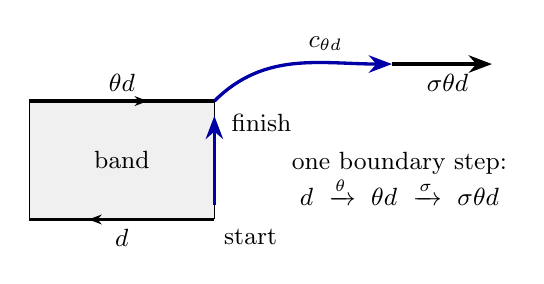
\begin{tikzpicture}[>=Stealth,scale=.94,every node/.style={font=\small}]
 \fill[gray!12] (0,0) rectangle (2.5,1.6);
 \draw (0,0)--(0,1.6) (2.5,0)--(2.5,1.6);
 \draw[very thick] (0,0)--(2.5,0) (0,1.6)--(2.5,1.6);
 \draw[->] (1.6,0)--(.8,0);
 \draw[->] (.8,1.6)--(1.6,1.6);
 \node[below] at (1.25,0) {$d$};
 \node[above] at (1.25,1.6) {$\theta d$};
 \node at (1.25,.8) {band};
 \node[below right] at (2.5,0) {start};
 \node[right] at (2.6,1.3) {finish};
 \draw[blue!65!black,very thick,->] (2.5,.2)--(2.5,1.4);
 \draw[blue!65!black,very thick,->] (2.5,1.6) to[out=45,in=180] (4.9,2.1);
 \node[above] at (4,2.15) {$c_{\theta d}$};
 \draw[very thick,->] (4.9,2.1)--(6.25,2.1);
 \node[below] at (5.65,2.1) {$\sigma\theta d$};
 \node[align=center] at (5,.55) {one boundary step:\\$d\ \xrightarrow{\theta}\ \theta d
 \ \xrightarrow{\sigma}\ \sigma\theta d$};
\end{tikzpicture}
\caption{The slot arrows follow the oriented boundaries of the word disks.
The blue path follows the boundary of the attached surface. The paired
slots have opposite traversal signs; the corner encountered after the band
is $c_{\theta d}$.}
\label{fig:boundary}
\end{figure}

There are $2k$ disks and $nk$ bands. If $q$ is the number of boundary
circles, the Euler characteristic gives
\begin{equation}\label{eq:euler}
 2-q=2k-nk,\qquad q=nk-2k+2.
\end{equation}
In particular $q\geq1$: the surface has nonempty boundary along its corners.

We will assign a small real phase $\eta_z$ to each boundary circle, with
$\sum_z\eta_z=0$. The phases will let us approach the spectral cut from
opposite sides on the trivial and possibly nontrivial boundary circles.
They can be realized by numbers $\gamma_d\in\R$
satisfying
\begin{equation}\label{eq:flows}
 \gamma_{\theta d}=-\gamma_d,\qquad
 \sum_{d\in z}\gamma_d=\eta_z.
\end{equation}
To see this, form a graph whose vertices are the cycles of $\sigma\theta$
and whose edges are the pairs $\{d,\theta d\}$. The graph is connected:
connectedness of $\Sigma$ makes $\langle\sigma,\theta\rangle$ transitive on
$D$, and this group equals $\langle\sigma\theta,\theta\rangle$.
On a spanning tree, any assignment of total sum zero is the divergence of
a real edge flow. For completeness, remove a leaf, put its required value
on its end of the incident edge and its negative on the other end, and
adjust the value required at the adjacent vertex. The final vertex has
value zero. Set all other edge flows to zero, including loops. This gives
\eqref{eq:flows}; if $q=1$, take every $\gamma_d=0$.

\subsection{An upper bound obtained by mixing the disks}

Use the algebra $M_{2nk}(\mathcal M)$ and its trace from
Section~\ref{sec:phase}, with matrix coordinates indexed by $D$.
On $\C^D\otimes\ell^2(A)$ define
\begin{align}\label{eq:shifts}
 S(e_d\otimes v)&=e_{\sigma d}\otimes L(c_d^{-1})v, &
 \Theta(e_d\otimes v)&=e^{2\pi i\gamma_d}e_{\theta d}\otimes v.
\end{align}
Both operators are unitary; \eqref{eq:flows} gives $\Theta^2=I$.
The product $S\Theta$ follows the boundary permutation $\sigma\theta$.
Its coefficient weights act on the left, so a complete circuit multiplies
the inverse corner labels in reverse order, giving the inverse boundary word.
We regard scalar matrices on $\C^D$ as elements of this algebra by tensoring
with the identity. For a scalar orthogonal projection $Q$,
$\tau_{2nk}(Q\otimes I)=\operatorname{rank}Q$, since $\tau(I)=1$.

Number the disks of each kind by $1,\ldots,k$. At each slot index $i$,
write $e_{+,i}(u)$ and $e_{-,i}(u)$ for the positive- and negative-disk
arrays with coefficient vector $u\in\C^k$. Given $X\in\U(k)$, put
\begin{equation}\label{eq:mixing}
 J e_{+,i}(u)=e_{-,i}(Xu),\qquad
 J e_{-,i}(u)=e_{+,i}(X^{-1}u).
\end{equation}
This scalar operator is a unitary involution. The corner convention gives
\begin{align*}
 S(e_{+,i}(u)\otimes v)&=e_{+,i+1}(u)\otimes L(a_i^{-1})v,\\
 S(e_{-,i}(u)\otimes v)&=e_{-,i-1}(u)\otimes L(a_{i-1})v.
\end{align*}
The same coefficient weight acts on all $k$ disks of a given kind.
Consequently $JSJ=S^{-1}$: on a positive array both sides shift to $i-1$
with weight $L(a_{i-1})$, and on a negative array both shift to $i+1$
with weight $L(a_i^{-1})$. Thus $SJ$ is a self-adjoint unitary. It exchanges
disk kinds, so its trace is zero. Its negative spectral projection
$(I-SJ)/2$ has trace $nk$, and hence
\begin{equation}\label{eq:phaseSJ}
 \ell(SJ)=\frac{nk}{2}.
\end{equation}

We now choose $X$ to make $J\Theta$ have a large fixed space. Let
$V_+$ and $V_-$ be the scalar coordinate spaces of slots with positive
and negative traversal signs. Each has dimension $nk$. Both $J$ and
$\Theta$ exchange them. In $V_+$, the block at index $i$ consists of
positive disks when $s_i=1$ and negative disks when $s_i=-1$; in $V_-$,
use the opposite kind. Order each block by disk number. In these bases
$\Theta:V_+\to V_-$ is a fixed matrix $P\in\U(nk)$, while $J:V_-\to V_+$
is $\diag(X^{-s_1},\ldots,X^{-s_n})$. Thus
\begin{equation}\label{eq:traversalblock}
 (J\Theta)|_{V_+}=\diag(X^{-s_1},\ldots,X^{-s_n})P.
\end{equation}
Lemma~\ref{lem:fixed}, applied to the signs $-s_i$, supplies $X$ for which
this block has at least $k$ fixed directions. Moreover,
$J(J\Theta)J=(J\Theta)^{-1}$, and $J$ exchanges $V_+$ and $V_-$.
The other block therefore also has at least $k$ fixed directions.

The eigenvalues of the scalar unitary $J\Theta$ are paired with their
inverses, with multiplicities. Since
$h(\lambda)+h(\lambda^{-1})=1$ for $\lambda\ne1$ and both terms vanish
at $1$, we obtain
\begin{equation}\label{eq:phaseJTheta}
 \ell(J\Theta)=\frac{2nk-\dim\ker(J\Theta-I)}{2}\leq nk-k.
\end{equation}
Apply Lemma~\ref{lem:phase} to $S\Theta=(SJ)(J\Theta)$:
\begin{equation}\label{eq:upper}
 \ell(S\Theta)\leq\frac32 nk-k.
\end{equation}
This bound holds for every choice of the boundary phases in
\eqref{eq:flows}. The choice of $X$ may depend on those phases.

\subsection{Computing the phase along boundary circles}

We compute the same trace directly from the boundary cycles. On a cycle
$z=(d_1,\ldots,d_{d_z})$, one circuit of $S\Theta$ starting at $d_1$ has
weight
\[
 e^{2\pi i\eta_z}
 L(c_{\theta d_{d_z}}^{-1})\cdots L(c_{\theta d_1}^{-1})
 =e^{2\pi i\eta_z}L(r_z^{-1}).
\]
Circuit weights at other starting points are unitary conjugates.
If $T_z$ is the restriction of $S\Theta$ to this cycle, then
\begin{equation}\label{eq:cyclephase}
 \ell(T_z)=\frac{d_z-1}{2}
   +\tau\bigl(h(e^{2\pi i\eta_z}L(r_z^{-1}))\bigr).
\end{equation}
Here and below $\ell$ uses the matrix trace of the appropriate size.
To prove the formula, let $d=d_z$ and $\zeta=e^{2\pi i/d}$.
Rephasing the successive coordinate vectors by $1,\zeta,\ldots,\zeta^{d-1}$
conjugates $T_z$ to $\zeta T_z$. For every $\lambda\in\T$ the exact identity
\[
 \sum_{j=0}^{d-1}h(\zeta^j\lambda)
   =\frac{d-1}{2}+h(\lambda^d)
\]
follows by listing the $d$ fractional parts; it also holds when
$\lambda^d=1$, because $h(1)=0$. Apply bounded Borel functional calculus
and take the trace. Each term on the left has trace $\ell(T_z)$.
The constant on the right has trace $d(d-1)/2$, and $T_z^d$ is diagonal
with $d$ conjugate circuit weights. Division by $d$ gives
\eqref{eq:cyclephase}.

\begin{proof}[Proof of Theorem~\ref{thm:planar}]
Let $z_0$ be the possibly nontrivial boundary circle.
We approach the phase cut from below on the trivial circles and from
above on $z_0$. Thus each trivial word contributes a limit of one, while
the exceptional word retains its nonnegative phase. For $\epsilon>0$ put
\[
 \eta_z=-\epsilon\quad(z\ne z_0),\qquad
 \eta_{z_0}=(q-1)\epsilon.
\]
These phases sum to zero. On each trivial circle the last term of
\eqref{eq:cyclephase} tends to $1$ as $\epsilon\downarrow0$.
On $z_0$ it tends to $\tau(h(L(r_{z_0}^{-1})))$: the fractional part
converges to its prescribed value from the nonnegative-shift side,
including at $1$, and the trace obeys bounded convergence.
For $q=1$ the exceptional phase is identically zero and there are no other
circles, so the same statement holds.

Since $\sum_zd_z=2nk$, summing \eqref{eq:cyclephase} and then using
\eqref{eq:euler} gives
\begin{align*}
 \lim_{\epsilon\downarrow0}\ell(S\Theta)
 &=\frac{2nk-q}{2}+q-1+\tau(h(L(r_{z_0}^{-1})))\\
 &=\frac32 nk-k+\tau(h(L(r_{z_0}^{-1}))).
\end{align*}
The uniform bound \eqref{eq:upper} forces the last term to vanish.
Faithfulness of $\tau$ and positivity of $h$ imply
$h(L(r_{z_0}^{-1}))=0$, hence $L(r_{z_0}^{-1})=I$ and $r_{z_0}=1$.
Only the uniform bound is used; no limiting choice of $X$ or $J$ is needed.
\end{proof}

\section{From a coefficient relation to a planar surface}
\label{sec:topology}

We now prove Theorem~\ref{thm:main}. The construction has two steps. A
finite product of conjugates of the relator gives a punctured disk with
paired bands. We then remove its connected band surfaces from the inside
out, applying Theorem~\ref{thm:planar} at each step.
The relation-to-surface interpretation is also described in
\cite[preprint Section 2, especially Example 2.5]{Chen2026}. We retain the finite
domain and the original coefficient map explicitly in the construction.

\begin{proof}[Proof of Theorem~\ref{thm:main}]
Cyclically conjugating the relator does not change its normal closure.
Since its total $t$-exponent is $\pm1$, it has a cyclic expression beginning
with a $t$-letter. Splitting powers of $t$ into individual letters gives
\eqref{eq:word}; identity coefficients are allowed. Suppose that
$g\in A$ belongs to the normal closure of $w$ in $A*\langle t\rangle$.
Then, for some finite $r$,
\begin{equation}\label{eq:normal-closure-product}
 g=\prod_{j=1}^{r} b_jw^{\varepsilon_j}b_j^{-1},
 \qquad b_j\in A*\langle t\rangle,\quad
 \varepsilon_j\in\{1,-1\}.
\end{equation}
If $r=0$, then $g=1$. Henceforth assume $r>0$.

\paragraph{Realizing the relation.}
Choose a based CW presentation space $Y$ with $\pi_1(Y)=A$. Such a space
exists for every group: take one loop $x_a$ for each $a\in A$ and attach
two-cells imposing $x_1=1$ and $x_ax_b=x_{ab}$. These relations identify
its fundamental group with $A$; see also
\cite[Corollary 1.28]{Hatcher2002}. Thus
$\pi_1(Y\vee\T)=A*\langle t\rangle$, with the added circle representing
$t$. All subsequent triangulations concern a finite planar domain.

Let $\Delta$ be a polygonal disk, and remove the interiors of $r$ disjoint
polygonal disks to obtain a planar surface $P$. There is a continuous map
\[
 f:P\longrightarrow Y\vee\T
\]
whose outer boundary is a based loop in $Y$ representing $g$, and whose
$j$th inner boundary reads $w^{\varepsilon_j}$ when oriented as the
boundary of its missing disk. To construct it, join marked points on the
inner circles to a common outer basepoint by cutting arcs that are otherwise
disjoint. Order the arcs so that the outer loop represents the ordered
product of the conjugated missing-disk loops, and map the $j$th arc to a
path representing $b_j$. Use chosen based coefficient loops in $Y$ and
one monotone traversal of $\T$, affine in angle, for each $t^{\pm1}$;
on an inverse relator, reverse the chosen paths in reverse order.
Cutting along the arcs gives a
disk whose boundary path is nullhomotopic by
\eqref{eq:normal-closure-product}. Extend over that disk and reglue the
matching copies of the arcs. This uses the equality in
$\pi_1(Y\vee\T)$, before imposing the relator $w$.

Write $u:P\to\T$ for the projection of $f$ that collapses $Y$, and
$v:P\to Y$ for the projection that collapses $\T$. The boundary map $u$
is constant on the outer circle and on every coefficient interval, and
traverses $\T$ once on each $t$-letter interval.

\paragraph{Extracting bands while retaining the original map.}
Identify $\T$ with $\mathbb R/\Z$, with wedge point $0$. Approximate
$u$, relative to the boundary, by a map $u'$ that is piecewise affine in
local angle coordinates, with uniform circle distance less than $1/12$.
Here is a direct construction. Subdivide the boundary so that its angle
maps are affine on each edge, and choose a sufficiently fine finite
triangulation of $P$. By uniform continuity, the image under $u$ of each
triangle lies in an arbitrarily short arc. Lift to angles on each triangle
and interpolate the vertex values affinely. The lifts on shared edges
differ by an integer, so the resulting circle maps agree there. On boundary
edges the interpolation equals $u$. Finer triangulations make the uniform
error arbitrarily small. Only the compact surface $P$ and its circle map
have been triangulated.

Choose an angle $z\in(1/3,2/3)$ outside the images of all vertices. The
level $u'^{-1}(z)$ is a finite disjoint union of polygonal circles and
properly embedded polygonal arcs: within each triangle it is a line
segment or empty, and it misses every vertex. Because $u'=u$ on the
boundary, each $t$-letter interval contains exactly one arc endpoint;
there are no other endpoints. Ignore the closed level circles.

The circle orientation coorients the level arcs. Their endpoints have
opposite crossing signs along the induced boundary orientation of $P$.
The missing-disk orientation reverses this boundary orientation at both
ends, so each arc pairs opposite $t$-letter signs in the word-disk
readings. This remains true for an arc with both ends on the same disk.

At every point of the level, the original value $u$ has distance greater
than $1/4$ from the wedge point. Consequently the original map $f$ takes
an open neighborhood of the level into $\T\setminus\{0\}$, and $v$ is
identically the basepoint there. Take pairwise disjoint thin rectangular
neighborhoods of the level arcs inside this neighborhood. They give bands
meeting the missing-disk boundaries in small intervals inside the
corresponding $t$-letter intervals. Thus $v$ is exactly constant throughout
every band.

Each small attachment interval is now a slot, with the sign of its
original $t$-letter. Between consecutive slots, the projected boundary
path consists of the original coefficient loop together with constant
pieces from the adjacent $t$-intervals. Its label in $A$ is therefore
unchanged. In particular positive disks have the corners $a_i$, and
negative disks have the reversed corners $a_i^{-1}$. This observation
allows the geometric attachment slots to be smaller than the original
letter intervals.

\paragraph{Removing the planar components.}
Put the missing disks back into $\Delta$ as word disks and adjoin all
the bands. Their union is a finite compact planar surface $S$, possibly
disconnected. Each component contains a word disk, every slot is used
once, and the paired signs are opposite. Its orientation is induced from
the plane, so it satisfies the disk-and-band hypotheses of
Theorem~\ref{thm:planar}. Along its boundary, $v$ reads exactly the
corner words from that theorem: band sides and remaining pieces of
$t$-intervals are constant in $Y$.

The nonexterior boundary words of an arbitrary component need not yet be
trivial, because other components may lie inside them. We therefore choose
an innermost component as follows. Every connected planar component $C$
has a unique exterior boundary circle; let $D(C)$ be the closed Jordan
disk it bounds. Its other boundary circles bound the inner complementary
disks of $C$. Among the finitely many $D(C)$ choose one minimal under
inclusion. No inner complementary disk of this $C$ contains another
component: such a component would have its exterior disk strictly inside
$D(C)$, contradicting minimality.

Each inner complementary disk of $C$ therefore contains no word disks.
It already carries the map $v$ to $Y$, so its boundary word is trivial in
$A$. Theorem~\ref{thm:planar} makes the exterior boundary word trivial
as well. Hence its actual boundary loop under $v$ is nullhomotopic in
$Y$. Fill all of $D(C)$ by a map to $Y$ agreeing with that boundary loop,
and discard the word disks and bands of $C$.

We continue to write $v$ for the resulting coefficient map.
This replacement changes nothing outside $D(C)$ and affects no other
component. It leaves a continuous $Y$-map outside the remaining word-disk
interiors, with the same corner readings and constant remaining bands.
That is precisely the invariant needed to repeat the argument; no further
circle approximation is required. Each step removes a component. After
finitely many steps, the original outer loop extends over $\Delta$ in
$Y$. Thus $g=1$ in $A$, proving the claimed injectivity.
\end{proof}

\bibliographystyle{plain}
\bibliography{references}
\end{document}
